%\documentclass[twoside,twocolumn,spanish]{article}
\documentclass{article}
\usepackage[T1]{fontenc}
\usepackage[utf8]{inputenc}
\usepackage{graphicx}
\usepackage[spanish]{babel}
\usepackage{amssymb,amsmath,geometry,multicol,spalign,hyperref}
\setlength\columnsep{20pt}
\usepackage[usenames,dvipsnames]{xcolor}
\usepackage{tikz,mathtools}
\usepackage{pgfplots}
\pgfplotsset{width=5cm,compat=1.12}
\usepgfplotslibrary{fillbetween}

\title{Ondas estacionarias en una cuerda con extremos fijos}
\author{Andoni Latorre Galarraga \\ \href{mailto:alatorre73@alumno.uned.es}{alatorre73@alumno.uned.es}}
\date{}
\begin{document}

\maketitle
\begin{abstract}

\end{abstract}

\begin{multicols}{2}

\section*{Fundamento Teórico}
Si $E(x,t)$ nos da la posición vertical de una cuerda en el punto $x$ en el instante $t$ y esta cuerda está sometida a una fuerza tangencial $T$, entonces se satisface la siguiente ecuación:
$$
\frac{\partial^2 E}{\partial t^2} = \frac{T}{\mu}\frac{\partial^2 E}{\partial x^2}
$$
donde $\mu$ es la densidad lineal de la cuerda. Si la cuerda tiene longitud $l$ y se fijan los extremos, es decir, $E(0,t)=E(l,t)=0$ Entonces las soluciones a la ecuación diferencial son:
$$
E(x,t)= 2E_0 \sen\left(\frac{2\pi x}{\lambda_n}\right)\cos\left(2\pi f_n t\right)
$$
$$
\lambda_n = \frac{2l}{n} \quad f_n = \frac{n}{2l}v \quad v=\sqrt{\frac{T}{\mu}}
$$
\section*{Dispositivo Experimental}
Un extremo de la cuerda se fija a un vibrador mecanico. El otro extremo, se pasa por una polea y se le cuelga una masa, $m$. A continuación, se muestra un esquema para $n = 4$.
\begin{center}
  \begin{tikzpicture}
    \draw[fill=gray] (0,0) -- (0.3,0) -- (0.3,0.3) -- (0,0.3) -- (0,0);
    \draw (0.3,0.15) sin (0.8,0.25) cos (1.3,0.15) sin (1.8,0.05) cos (2.3,0.15) sin (2.8,0.25) cos (3.3,0.15) sin (3.8,0.05) cos (4.3,0.15);
    \draw (0.3,0.15) sin (0.8,0.05) cos (1.3,0.15) sin (1.8,0.25) cos (2.3,0.15) sin (2.8,0.05) cos (3.3,0.15) sin (3.8,0.25) cos (4.3,0.15);
    \draw[stealth-stealth] (0.3,-0.2) -- (4.3,-0.2);
    \draw[stealth-stealth] (0.3,0.4) -- (1.3,0.4);
    \draw[fill=gray] (4.3,0) circle (0.15);
    \draw (4.45,0) -- (4.45,-0.5);
    \node at (2.3,-0.4){$l$};
    \node at (0.8,0.7){$\frac{\lambda}{2}$};
    \draw[fill=gray!40] (4.2,-0.5) -- (4.7,-0.5) -- (4.7,-1) -- (4.2,-1) -- (4.2,-0.5);
    \node at (4.45,-0.75){$m$};
  \end{tikzpicture}
\end{center}
También se utliza una luz estroboscópica para poder ver  la cuerda al sicronizarse la frecuencia de la luz con la de la cuerda.
\begin{center}
  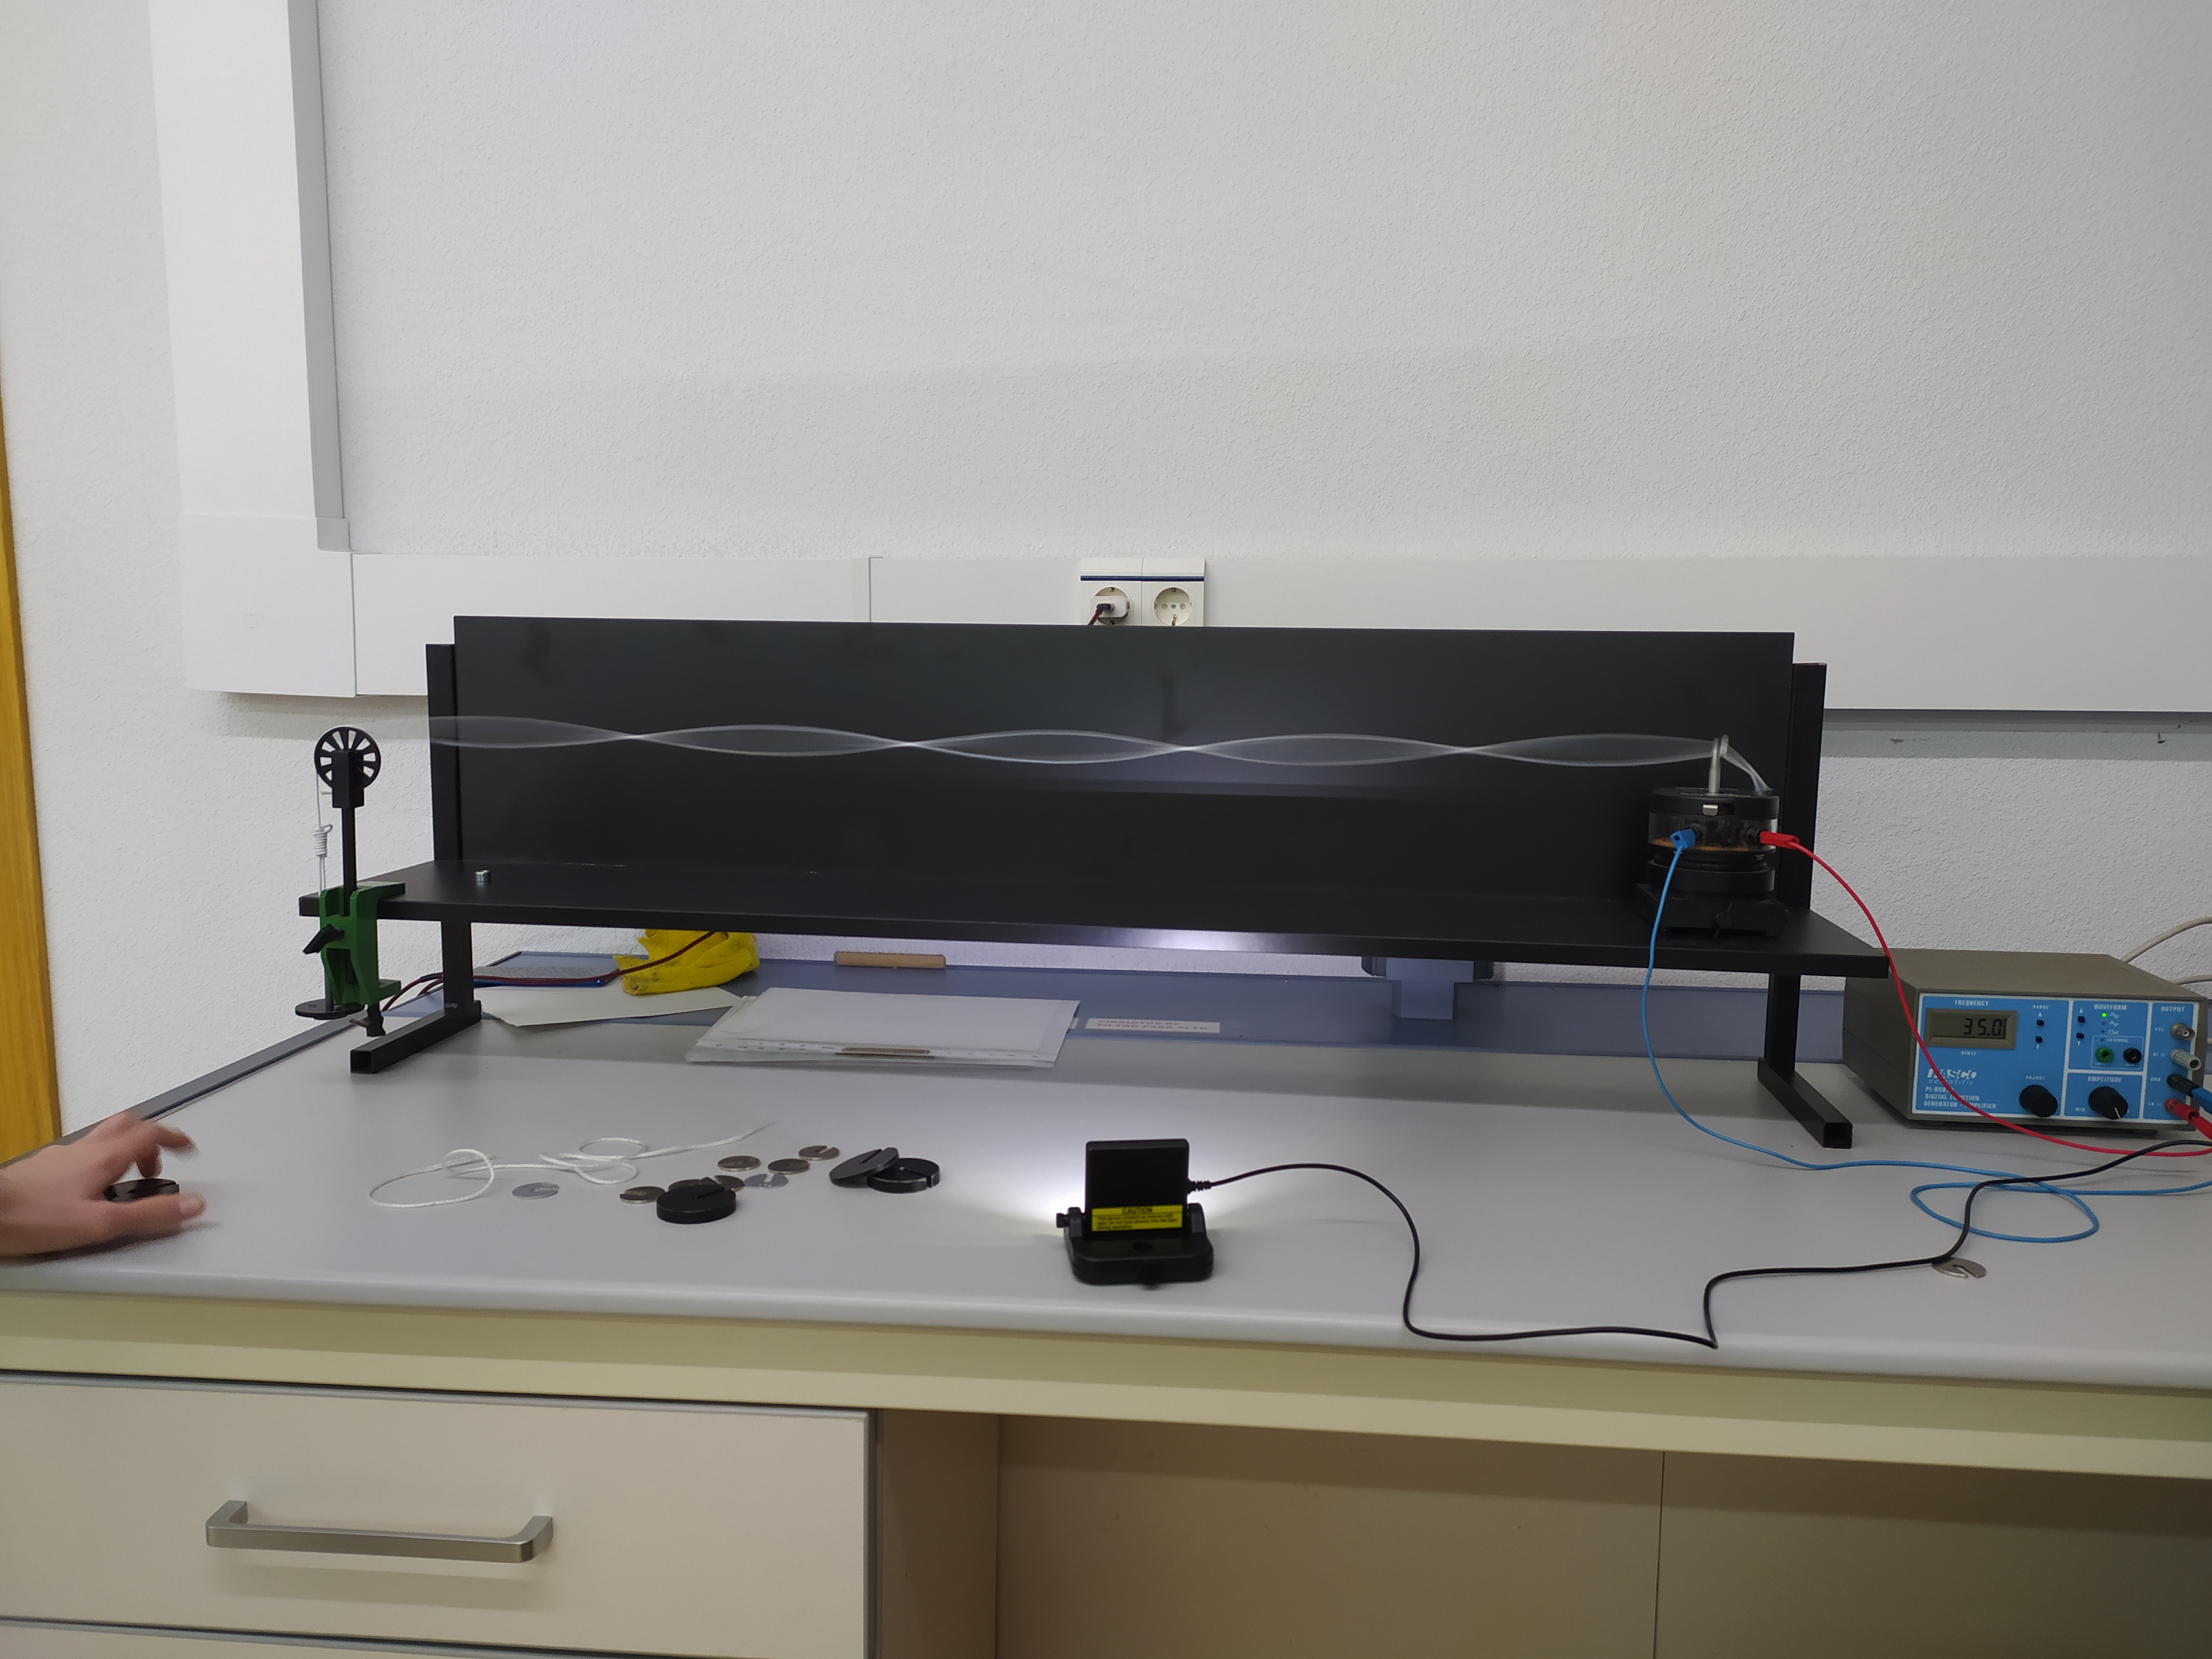
\includegraphics[width=0.45\textwidth]{figures/montaje.png}\\
  Figura 1: Dispositivo experimental.
\end{center}

\section*{Procedimiento y Resultados}
\subsection*{Cuerda rígida}
Primero hemos fijado $l=(1.05 \pm 0.01)$m. Tambien hemos medido la cuerda completa $1.5$m y la hemos pesado $2.0$g. Obteniendo una densidad de $1.33\times10^{-3}$Kg/m. Para el valor de $g$ tomaremos será de $9,847$ms\textsuperscript{-2}, obtenido de \cite{gravedad} sabiendo que la latitud del laboratorio es de unos $43.3305^\circ$. Hemos obtenido los valores de $\lambda/2$ y $f$ para 5 valores de $m$.
\end{multicols}
\begin{center}
  Tabla 1: Cuerda rígida.
  $$
  \begin{array}{|l|l|l|l|l|l|l|l|l|l|} \hline
    m\text{(kg)} & T\text{(N)} & n & v_{teo}\text{(m/s)} & f_{teo}\text{(Hz)} & \lambda_{teo}\text{(m)} & f_{exp}\text{(Hz)} & \lambda_{exp}\text{(m)} & v_{exp}\text{(m/s)} & v_{exp}^2\text{(m\textsuperscript{2}/s\textsuperscript{2})} \\ \hline \hline
    0.5143 & 5.06 & 1 & 61.71 & 29.38 & 2.1 & 31.0 & 2.08 & 65.1 & 4238.01  \\ \hline
     &  & 2 &  & 58.77 & 1.05 & 59.0 & 1.05 & 61.95 & 3837.8  \\ \hline
     &  & 3 &  & 88.15 & 0.7 & 90.5 & 0.7 & 63.35 & 4013.22  \\ \hline
     &  & 4 &  & 117.54 & 0.525 & 113.0 & 0.53 & 59.33 & 3519.46  \\ \hline \hline
    0.2623 & 2.58 & 1 & 44.07 & 20.98 & 2.1 & 19.2 & 2.1 & 40.32 & 1625.7  \\ \hline
     &  & 2 &  & 41.97 & 1.05 & 39.6 & 1.07 & 41.58 & 1728.9  \\ \hline
     &  & 3 &  & 62.95 & 0.7 & 65.3 & 0.714 & 45.71 & 2089.4  \\ \hline
     &  & 4 &  & 83.94 & 0.525 & 73.8 & 0.54 & 38.74 & 1501.18  \\ \hline \hline
    0.1256 & 1.24 & 2 & 30.49 & 29.04 & 1.05 & 29.3 & 1.08 & 30.77 & 946.49  \\ \hline
     &  & 3 &  & 43.56 & 0.7 & 41.8 & 0.72 & 29.26 & 856.15  \\ \hline
     &  & 4 &  & 58.08 & 0.525 & 56.6 & 0.55 & 29.72 & 882.98  \\ \hline
     &  & 5 &  & 72.61 & 0.42 & 75.7 & 0.42 & 31.79 & 1010.86  \\ \hline \hline
    0.1841 & 1.81 & 2 & 36.92 & 35.16 & 1.05 & 36.2 & 1.08 & 38.01 & 1444.76  \\ \hline
     &  & 3 &  & 52.74 & 0.7 & 53.7 & 0.72 & 37.59 & 1413.01  \\ \hline
     &  & 4 &  & 70.32 & 0.525 & 68.6 & 0.52 & 36.02 & 1297.08  \\ \hline
     &  & 5 &  & 87.9 & 0.42 & 77.9 & 0.44 & 32.72 & 1070.47  \\ \hline \hline
    0.0616 & 0.61 & 1 & 21.36 & 10.17 & 2.1 & 11.2 & 2.1 & 23.52 & 553.19  \\ \hline
     &  & 2 &  & 20.34 & 1.05 & 21.7 & 1.04 & 22.79 & 519.16  \\ \hline
     &  & 3 &  & 30.51 & 0.7 & 30.1 & 0.75 & 21.07 & 443.94  \\ \hline
     &  & 4 &  & 40.68 & 0.525 & 37.2 & 0.548 & 19.53 & 381.42  \\ \hline
    \end{array}
  $$
\end{center}
\begin{multicols}{2}
Representando $v^2$ frente a $T$. Y calculando la recta de regresión $y = ax+b$. Se tiene que
$$
\mu = \frac{1}{a} \quad \epsilon_{\mu} = \frac{\epsilon_a}{a^2}
$$
\begin{center}
  \includegraphics[width=0.45\textwidth]{figures/regresión1.png}\\
  Figura 2: Cuerda rígida.
\end{center}
La densidad obtenida es:
$$
\mu = (1.30\pm0.005)\times 10^{-3}\text{Kg/m}
$$

\subsection*{Cuerda elástica}
El procedimiento es análogo al de la cuerda rígida. La cuerda mide $1.2$m y pesa 7.0g. Se tiene una densidad de $5.83\times10^{-3}$Kg/m.
\begin{center}
  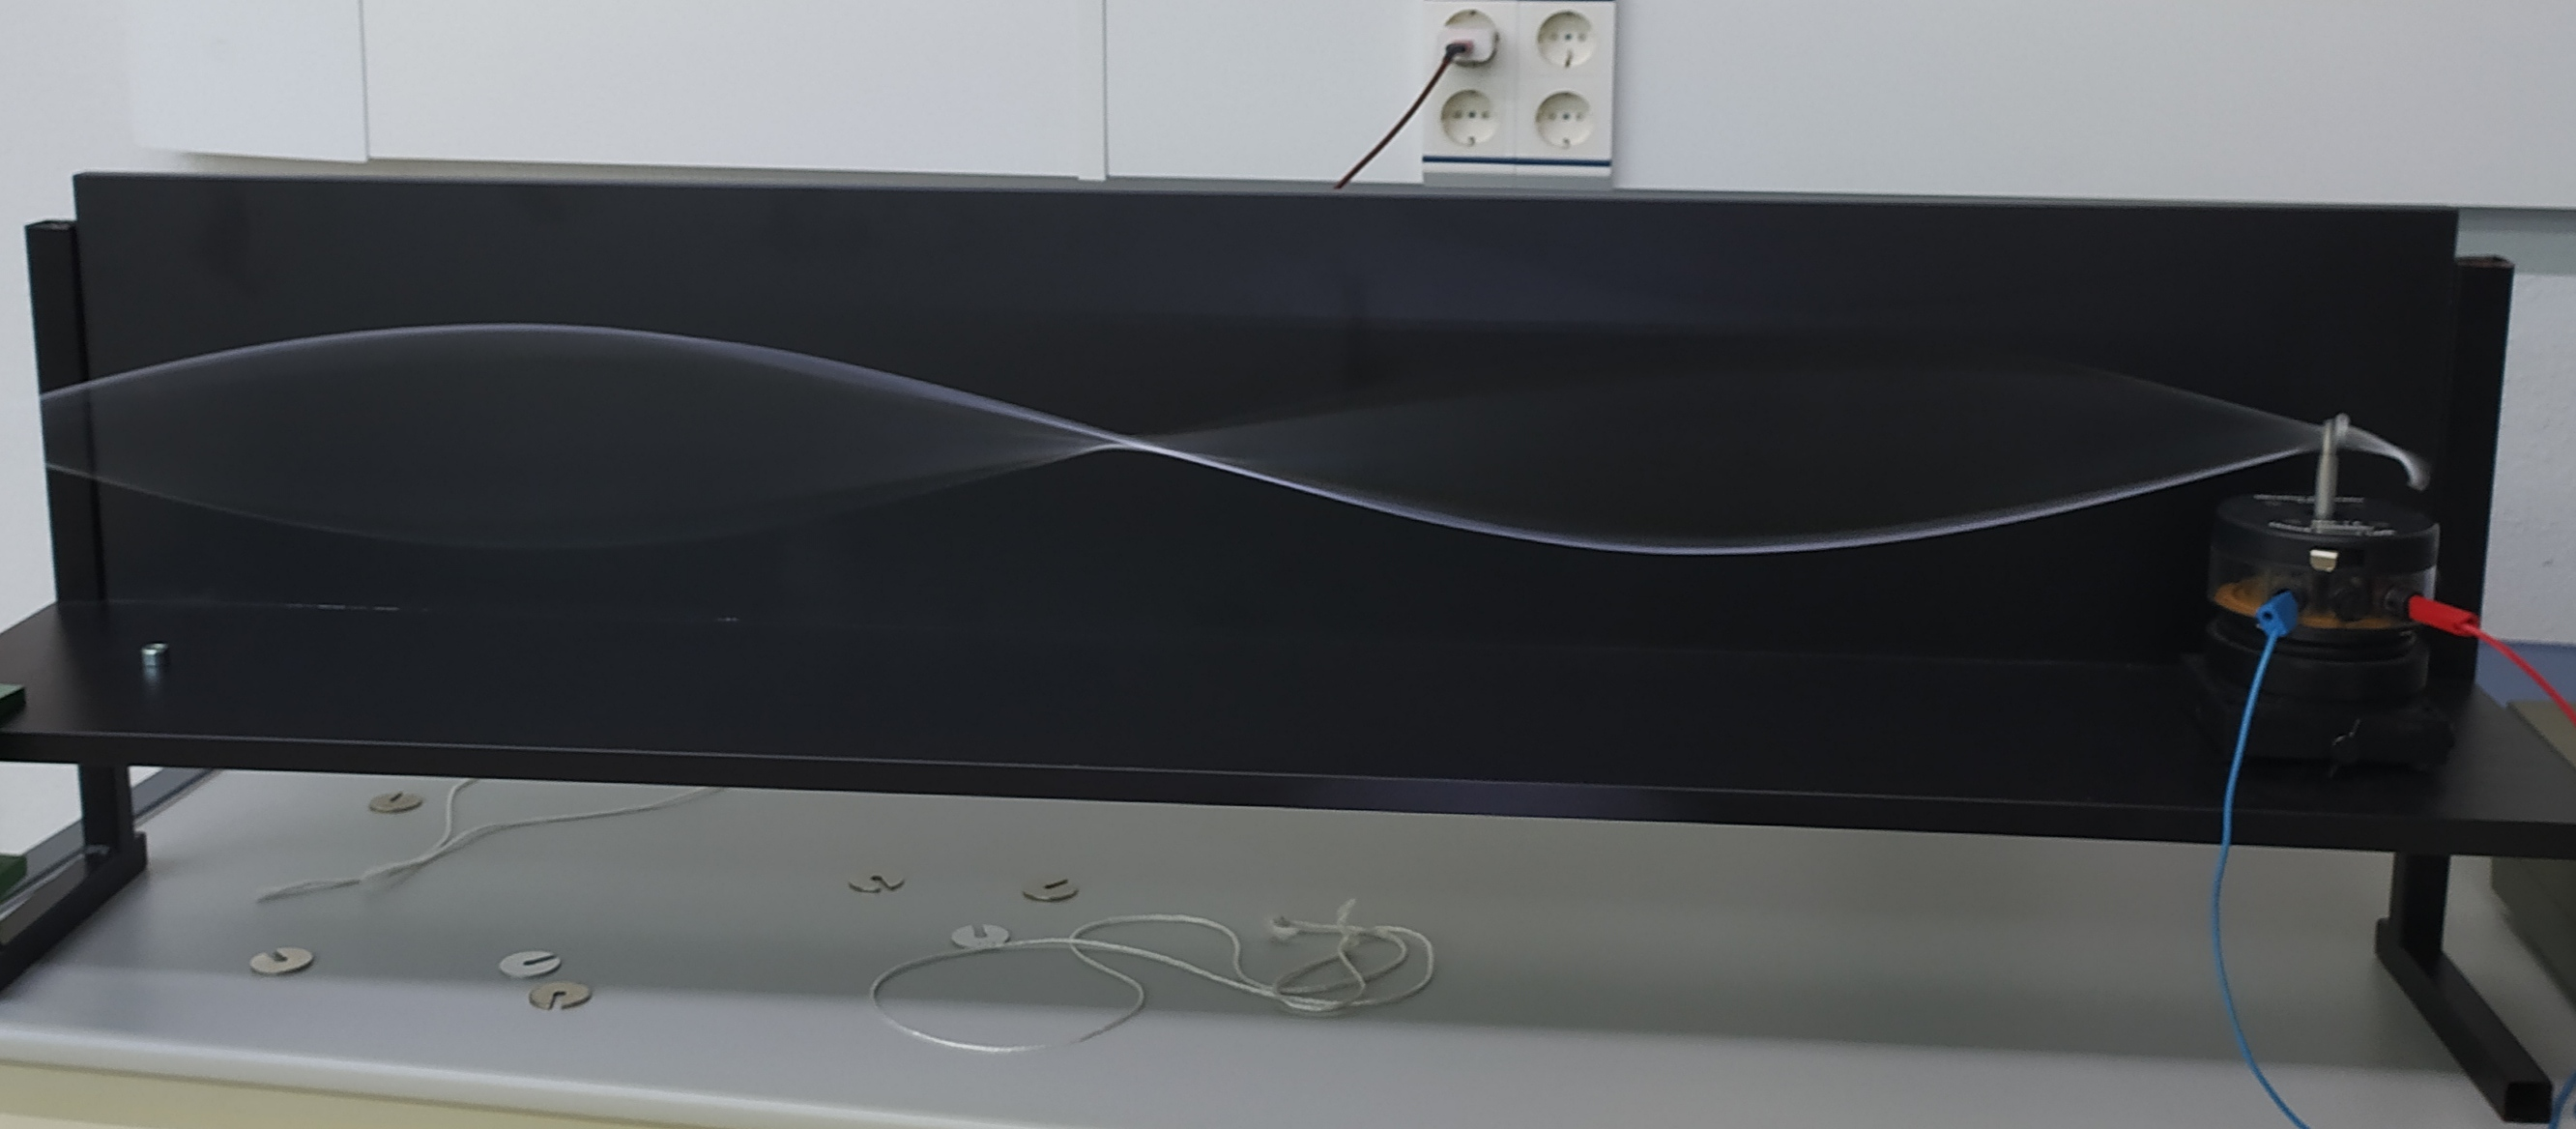
\includegraphics[width=0.45\textwidth]{figures/n2.png}
  Figura 3: Cuerda elástica con $n=2$.
\end{center}
\end{multicols}
\begin{center}
  Tabla 2: Cuerda elástica.
  $$
  \begin{array}{|l|l|l|l|l|l|l|l|l|l|} \hline
    m\text{(kg)} & T\text{(N)} & n & v_{teo}\text{(m/s)} & f_{teo}\text{(Hz)} & \lambda_{teo}\text{(m)} & f_{exp}\text{(Hz)} & \lambda_{exp}\text{(m)} & v_{exp}\text{(m/s)} & v_{exp}^2\text{(m\textsuperscript{2}/s\textsuperscript{2})} \\ \hline \hline
    0.0616 & 0.61 & 2 & 10.2 & 9.71 & 1.05 & 15.3 & 1.08 & 16.07 & 258.08  \\ \hline
     &  & 3 &  & 14.57 & 0.7 & 22.5 & 0.72 & 15.75 & 248.06  \\ \hline
     &  & 4 &  & 19.43 & 0.525 & 32.0 & 0.534 & 16.8 & 282.24  \\ \hline
     &  & 5 &  & 24.29 & 0.42 & 35.0 & 0.42 & 14.7 & 216.09  \\ \hline \hline
    0.1615 & 1.59 & 1 & 16.52 & 7.86 & 2.1 & 9.1 & 2.1 & 19.11 & 365.19  \\ \hline
     &  & 2 &  & 15.73 & 1.05 & 20.4 & 1.05 & 21.42 & 458.82  \\ \hline
     &  & 3 &  & 23.59 & 0.7 & 28.9 & 0.73 & 20.23 & 409.25  \\ \hline
     &  & 4 &  & 31.46 & 0.525 & 37.6 & 0.54 & 19.74 & 389.67  \\ \hline \hline
    0.2629 & 2.59 & 2 & 21.07 & 20.07 & 1.05 & 20.4 & 1.04 & 21.42 & 458.82  \\ \hline
     &  & 3 &  & 30.1 & 0.7 & 30.6 & 0.73 & 21.42 & 458.82  \\ \hline
     &  & 4 &  & 40.14 & 0.525 & 40.8 & 0.54 & 21.42 & 458.82  \\ \hline
     &  & 5 &  & 50.17 & 0.42 & 51.0 & 0.434 & 21.42 & 458.82  \\ \hline \hline
    0.3136 & 3.09 & 1 & 23.01 & 10.96 & 2.1 & 11.6 & 2.1 & 24.36 & 593.41  \\ \hline
     &  & 2 &  & 21.92 & 1.05 & 23.5 & 1.05 & 24.68 & 608.86  \\ \hline
     &  & 3 &  & 32.88 & 0.7 & 34.0 & 0.73 & 23.8 & 566.44  \\ \hline
     &  & 4 &  & 43.84 & 0.525 & 44.6 & 0.55 & 23.42 & 548.26  \\ \hline \hline
    0.3622 & 3.57 & 1 & 24.73 & 11.78 & 2.1 & 13.8 & 2.1 & 28.98 & 839.84  \\ \hline
     &  & 2 &  & 23.56 & 1.05 & 27.6 & 1.06 & 28.98 & 839.84  \\ \hline
     &  & 3 &  & 35.33 & 0.7 & 41.5 & 0.71 & 29.05 & 843.9  \\ \hline
     &  & 4 &  & 47.11 & 0.525 & 55.4 & 0.53 & 29.09 & 845.94  \\ \hline
    \end{array}
  $$
\end{center}
\begin{multicols}{2}
  Representando $v^2$ frente a $T$. Y calculando la recta de regresión $y = ax+b$. Se tiene que
$$
\mu = \frac{1}{a} \quad \epsilon_{\mu} = \frac{\epsilon_a}{a^2}
$$
\begin{center}
  \includegraphics[width=0.45\textwidth]{figures/regresión2.png}\\
  Figura 4: Cuerda elástica.
\end{center}
La densidad obtenida es:
$$
\mu = (5.8\pm0.6)\times 10^{-3}\text{Kg/m}
$$
\section*{Conclusiones}
En las tablas 1 y 2 se observa que las predicciones teóricas se acercan mucho a las observaciones experimentales, confirmando las ecuaciones teóricas. Por otra parte, las mediciones indirectas de las densidades de las cuerdas son muy acertadas, tienen poco error y coinciden con las mediciones directas de las densidades.
\begin{thebibliography}{1}

  \bibitem{manual}Manual de la asignatura. Versión 3.7

  \bibitem{web}\url{https://uned-labo.netlify.app/practicas/te/7_practica_ondas_estacionarias/prak7.html} 17/0/2022

  \bibitem{gravedad}\url{https://www.sensorsone.com/local-gravity-calculator/} 15/6/2022

\end{thebibliography}
\end{multicols}
\end{document}